% \documentclass[a4paper, conference, compsoc]{IEEEtran}
\documentclass[12pt,a4paper,colorinlistoftodos]{article}
% \documentclass[%
%     pdftex,
%     oneside,			% Einseitiger Druck.
%     12pt,				% Schriftgroesse
%     parskip=half,		% Halbe Zeile Abstand zwischen Absätzen.
% %	topmargin = 10pt,	% Abstand Seitenrand (Std:1in) zu Kopfzeile [laut log: unused]
%     headheight = 12pt,	% Höhe der Kopfzeile
% %	headsep = 30pt,	% Abstand zwischen Kopfzeile und Text Body  [laut log: unused]
%     headsepline,		% Linie nach Kopfzeile.
%     footsepline,		% Linie vor Fusszeile.
%     footheight = 16pt,	% Höhe der Fusszeile
%     abstracton,		% Abstract Überschriften
%     DIV=calc,		% Satzspiegel berechnen
%     BCOR=8mm,		% Bindekorrektur links: 8mm
%     headinclude=false,	% Kopfzeile nicht in den Satzspiegel einbeziehen
%     footinclude=false,	% Fußzeile nicht in den Satzspiegel einbeziehen
%     listof=totoc,		% Abbildungs-/ Tabellenverzeichnis im Inhaltsverzeichnis darstellen
%     toc=bibliography,	% Literaturverzeichnis im Inhaltsverzeichnis darstellen
% ]{scrreprt}	% Koma-Script report-Klasse, fuer laengere Bachelorarbeiten alternativ auch: scrbook


% Basic packages
\usepackage[T1]{fontenc}
\usepackage[utf8]{inputenc}
\usepackage[scaled]{beramono}
\usepackage[english,ngerman]{babel,varioref}
\usepackage{xcolor}
\usepackage{amsmath}

% Tables
\usepackage{booktabs}
\usepackage{multirow}
\usepackage{longtable}
% Graphics and Includes
\usepackage[pdftex]{graphicx}
\graphicspath{{assets/img/}}
\DeclareGraphicsExtensions{.pdf,.jpeg,.png,.jpg}
\usepackage{tikz}
\usetikzlibrary{arrows.meta,bending,automata,shapes}
\usepackage[underline=true,rounded corners=false]{pgf-umlsd}

% Reduce distance before caption
\usepackage[skip=5pt]{caption}
% Bibliography
\usepackage[backend=biber, isbn=false, doi=false, style=ieee]{biblatex}
\addbibresource{bibliography.bib}
\AtBeginBibliography{\raggedright}
%\nocite{*}

% Gossar z.a. für acronyme
% \usepackage[acronym]{glossaries}
% \makeglossaries
\usepackage[printonlyused]{acronym} % falls gewünscht kann die Option footnote eingefügt werden, dann wird die Erklärung nicht inline sondern in einer Fußnote dargestellt

% \section*{Abkürzungsverzeichnis}
\begin{acronym}[AAAAAAA]
    \acro{wysiwyg}[WYSIWYG]{What you see is what you get}
\end{acronym}

% Colors
\definecolor{ListingBackground}{HTML}{E6E6E6}
\definecolor{LinkColor}{HTML}{000000}


% Font
\usepackage[onehalfspacing]{setspace}
\usepackage{lmodern}
\usepackage[official]{eurosym}
\usepackage{enumitem}
\usepackage[locale=DE]{siunitx} % SI Units für Währungen
\DeclareSIUnit{\EUR}{\text{\euro}} % Beispielverwendung: \SI{10.10}{\EUR}

\usepackage[autostyle=true,german=quotes]{csquotes}
\usepackage{url}
\newcommand{\code}[1]{\texttt{#1}}

% Additional Setup
\usepackage[unicode=true,hypertexnames=false,colorlinks=true,linkcolor=LinkColor,citecolor=LinkColor,urlcolor=LinkColor,pdftex]{hyperref}

% Trennung von URLs im Literaturverzeichnis (große Werte [> 10000] verhindern die Trennung)
\defcounter{biburlnumpenalty}{10} % Strafe für Trennung in URL nach Zahl
\defcounter{biburlucpenalty}{500}  % Strafe für Trennung in URL nach Großbuchstaben
\defcounter{biburllcpenalty}{500}  % Strafe für Trennung in URL nach Kleinbuchstaben
\interfootnotelinepenalty=10000 % prevent all footnotes from breaking over a page.

% Configs
\setcounter{tocdepth}{1} % Limit table of contents to subsection
\sisetup{detect-weight=true, detect-family=true} % SI Units shall detect font weight and family
\setlist[description]{style=nextline} % Break definitions of terms to a new line (used by \begin{description} \item[foo] bar \end{description})
\renewcommand*{\bibfont}{\small}

%Hurenkinder und Schusterjungen vermeiden
\clubpenalty = 10000
\widowpenalty = 10000
\displaywidowpenalty = 10000

% Quellcode
\usepackage{listings}
\usepackage{float}
\usepackage{textcomp}
\lstset{
    inputpath=assets/listings,
    language=Java,			% Standardsprache des Quellcodes
    numbers=left,			% Zeilennummern links
    stepnumber=1,			% Jede Zeile nummerieren.
    numbersep=5pt,			% 5pt Abstand zum Quellcode
    numberstyle=\tiny,		% Zeichengrösse 'tiny' für die Nummern.
    breaklines=true,		% Zeilen umbrechen wenn notwendig.
    breakautoindent=true,	% Nach dem Zeilenumbruch Zeile einrücken.
    postbreak=\space,		% Bei Leerzeichen umbrechen.
    tabsize=2,				% Tabulatorgrösse 2
    basicstyle=\ttfamily\footnotesize, % Nichtproportionale Schrift, klein für den Quellcode
    showspaces=false,		% Leerzeichen nicht anzeigen.
    showstringspaces=false,	% Leerzeichen auch in Strings ('') nicht anzeigen.
    extendedchars=true,		% Alle Zeichen vom Latin1 Zeichensatz anzeigen.
    captionpos=b,			% sets the caption-position to bottom
    backgroundcolor=\color{ListingBackground}, % Hintergrundfarbe des Quellcodes setzen.
    xleftmargin=0pt,		% Rand links
    xrightmargin=0pt,		% Rand rechts
    frame=single,			% Rahmen an
    frameround=ffff,
    rulecolor=\color{darkgray},	% Rahmenfarbe
    fillcolor=\color{ListingBackground},
    keywordstyle=\color[rgb]{0.133,0.133,0.6},
    commentstyle=\color[rgb]{0.133,0.545,0.133},
    stringstyle=\color[rgb]{0.627,0.126,0.941},
    float,
    upquote=true
}


\colorlet{punct}{red!60!black}
\definecolor{delim}{RGB}{20,105,176}
\colorlet{numb}{magenta!60!black}

\lstdefinelanguage{json}{
    string=[s]{"}{"},
    stringstyle=\color{numb},
    literate=
     *{0}{{{\color{numb}0}}}{1}
      {1}{{{\color{numb}1}}}{1}
      {2}{{{\color{numb}2}}}{1}
      {3}{{{\color{numb}3}}}{1}
      {4}{{{\color{numb}4}}}{1}
      {5}{{{\color{numb}5}}}{1}
      {6}{{{\color{numb}6}}}{1}
      {7}{{{\color{numb}7}}}{1}
      {8}{{{\color{numb}8}}}{1}
      {9}{{{\color{numb}9}}}{1}
      {:}{{{\color{punct}{:}}}}{1}
      {,}{{{\color{punct}{,}}}}{1}
      {\{}{{{\color{delim}{\{}}}}{1}
      {\}}{{{\color{delim}{\}}}}}{1}
      {[}{{{\color{delim}{[}}}}{1}
      {]}{{{\color{delim}{]}}}}{1}
}

\lstdefinelanguage{yaml}{
  identifierstyle=\color{delim},
  sensitive=false,
  comment=[l]{\#},
  commentstyle=\color{purple}\ttfamily,
  stringstyle=\color{numb},
  morestring=[b]',
  morestring=[b]"
}

\lstloadlanguages{Python,Java,bash}



% Algorithmen (Pseudocode)
\usepackage[german,onelanguage,linesnumbered,ruled]{algorithm2e}
\newcommand\mycommfont[1]{\color{gray}\ttfamily{#1}}
\SetCommentSty{mycommfont}
% Useful tools
\usepackage{blindtext}
\usepackage{lipsum}
\usepackage[section]{placeins} % Prevent figures and tables to float to new section
\usepackage[obeyFinal,backgroundcolor=yellow,linecolor=black]{todonotes}


%Angaben zur Arbeit
\def\myTitel{Erlernen von Kundenpräferenzen in einer Wohnungsbörse}
\def\myArbeit{Programmentwurf}
\def\myFach{Maschinelles Lernen}
\def\myDatum{\today}
\def\myBetreuer{Prof. Dr. Dirk Reichardt}
\def\myGutachter{Strenger Gutachter}
\def\myBearbeitungszeit{Lange}
\def\myAbgabeort{Heilbronn}

%Angaben zur Person
\def\myAutor{Daniel Knecht, Lea Poletin}
\def\myDegree{Master Informatik}
\def\myInstitution{DHBW CAS, Bildungscampus 13, 74076 Heilbronn}
\def\myMatrikelnr{123456, 8514262}
\def\myKurs{TMINF17}
\def\myFirma{SAP SE}
\def\myFirmenort{Walldorf}
%\section*{Abkürzungsverzeichnis}
\begin{acronym}[AAAAAAA]
    \acro{wysiwyg}[WYSIWYG]{What you see is what you get}
\end{acronym}

\begin{document}


\title{\myTitel}
\author{\myAutor~(\myMatrikelnr)\\
    \small{\myFach}\\
    \small{\myDegree}\\
    \small{\myInstitution}
}
\date{\myDatum}

\begin{titlepage}
	\begin{longtable}{p{8.2cm} p{5.4cm}}
		% Firmenlogo
		&
		
\includegraphics[width=5.4cm]{casLogo}
	\end{longtable}
	\addtocounter{table}{-1}
    {\let\newpage\relax\maketitle}
    \thispagestyle{empty}
    % \vfill
    \begin{abstract}
Dieser Programmentwurf befasst sich mit der Problemstellung einer Wohnungsbörse.
Es werden Konzepte aus dem Bereich des \emph{Maschinellen Lernen} entwickelt
und eines dieser Konzepte implementiert.
Die Systeme erlernen die gegebene Bewertungsfunktion
umn anschließend neue Datensätze nach dem gleichen Schema zu bewerten.
\end{abstract}
\end{titlepage}
% \begin{titlepage}
	\begin{longtable}{p{8.2cm} p{5.4cm}}
		% Firmenlogo
		&
		
\includegraphics[width=5.4cm]{casLogo}
	\end{longtable}
	\addtocounter{table}{-1}
	\enlargethispage{20mm}
	\begin{center}
		\vspace*{12mm}	{\LARGE\textbf \myTitel }\\
		\vspace*{12mm}	{\large\textbf \myArbeit}\\
		% \vspace*{12mm}	\langdeckblattabschlusshinleitung\\
		\vspace*{3mm}		{\textbf \myDegree}\\
		\vspace*{12mm}	des Studiengangs \myKurs\\
    \vspace*{3mm}		am DHBW CAS\\
		\vspace*{12mm}	von\\
		\vspace*{3mm}		{\large\textbf \myAutor}\\
		\vspace*{12mm}	\myDatum\\
	\end{center}
	\vfill
	\begin{spacing}{1.2}
	\begin{tabbing}
		mmmmmmmmmmmmmmmmmmmmmmmmmm             \= \kill
		\textbf{Bearbeitungszeit}       \>  \myBearbeitungszeit\\
		\textbf{Matrikelnummer, Kurs}  \>  \myMatrikelnr, \myKurs\\
		\textbf{Firma}                  \>  \myFirma, \myFirmenort\\
		\textbf{Betreuer}               \>  \myBetreuer\\
		\textbf{Gutachter}              \>  \myGutachter
	\end{tabbing}
	\end{spacing}
\end{titlepage}

\pagenumbering{Roman}

% Sperrvermerk
% \thispagestyle{empty}
% Sperrvermerk direkt hinter Titelseite
\section*{Sperrvermerk}

\vspace*{2em}

Die vorliegende {\myArbeit} mit dem Titel {\itshape{} \myTitel{}\/}
enthält unternehmensinterne bzw. vertrauliche Informationen der {\myFirma},
ist deshalb mit einem Sperrvermerk versehen
und wird ausschließlich zu Prüfungszwecken am Studiengang
{\myDegree} der Dualen Hochschule Baden-Württemberg vorgelegt.
Sie ist ausschließlich zur Einsicht durch den zugeteilten Gutachter,
die Leitung des Studiengangs und ggf. den Prüfungsausschuss des Studiengangs
bestimmt.  Es ist untersagt,
\begin{itemize}
\item den Inhalt dieser Arbeit (einschließlich Daten, Abbildungen, Tabellen, Zeichnungen usw.) als Ganzes oder auszugsweise weiterzugeben,
\item Kopien oder Abschriften dieser Arbeit (einschließlich Daten, Abbildungen, Tabellen, Zeichnungen usw.) als Ganzes oder in Auszügen anzufertigen,
\item diese Arbeit zu veröffentlichen bzw. digital, elektronisch oder virtuell zur Verfügung zu stellen.
\end{itemize}
Jede anderweitige Einsichtnahme und Veröffentlichung – auch von Teilen der Arbeit – bedarf der vorherigen Zustimmung durch den Verfasser und {\myFirma}.

\vspace{3em}

\myAbgabeort, \myDatum
\vspace{4em}

\rule{6cm}{0.4pt}\\
\myAutor

% \newpage

% Erklärung
\thispagestyle{empty}

\section*{Selbstständigkeitserklärung}
\vspace*{2em}


Wir versicheren hiermit,
dass der {\myArbeit} mit dem Thema: {\itshape \myTitel } selbstständigverfasst und keine anderen
als die angegebenen Quellen und Hilfsmittel verwendet wurden.
Wir versicheren zudem, dass die eingereichte elektronische Fassung mit der gedruckten Fassung übereinstimmt.


\vspace{3em}
\noindent
\myAbgabeort, \myDatum
\\
\\
\noindent
\begin{tabular}{l l}
\rule{6cm}{0.4pt} &  \rule{6cm}{0.4pt}\\
\myAutorA         &  \myAutorB

\end{tabular}

\newpage


% \begin{abstract}
Dieser Programmentwurf befasst sich mit der Problemstellung einer Wohnungsbörse.
Es werden Konzepte aus dem Bereich des \emph{Maschinellen Lernen} entwickelt
und eines dieser Konzepte implementiert.
Die Systeme erlernen die gegebene Bewertungsfunktion
umn anschließend neue Datensätze nach dem gleichen Schema zu bewerten.
\end{abstract}
% \newpage

\pagestyle{plain}		% nur Seitenzahlen im Fuß

% Inhaltsverzeichnis
\begin{spacing}{1.1}
    \begingroup
        \pagestyle{empty}
        %für die Anzeige von Unterkapiteln im Inhaltsverzeichnis
        \setcounter{tocdepth}{2}

        \tableofcontents
        \clearpage
    \endgroup
\end{spacing}
\newpage

% Abkürzungsverzeichnis
\cleardoublepage
\section*{Abkürzungsverzeichnis}
\begin{acronym}[AAAAAAA]
    \acro{wysiwyg}[WYSIWYG]{What you see is what you get}
\end{acronym}


% Abbildungsverzeichnis
\cleardoublepage
\listoffigures

%Tabellenverzeichnis
\cleardoublepage
\listoftables

% Quellcodeverzeichnis
\cleardoublepage
\lstlistoflistings
\cleardoublepage

\listoftodos
\cleardoublepage


\pagenumbering{arabic}

\section{Einleitung}\label{sec:einleitung}
In diesem Programmentwurf wird das Problem \emph{Erlernen von Kundenpräferenzen in einer Wohnungsbörse}
bearbeitet. Gegeben sind zwei Datensätze: 
\begin{itemize}
    \item Datensatz zum Trainieren mit erwartetem Ergebnis
    \item Datensatz zum Testen ohne erwartetes Ergebnis
\end{itemize}

Die Datensätze beschreiben 22 Merkmale von Wohnungen die in einer Wohnungsbörse angeboten werden. \\
Zunächst werden die gegebenen Daten analysiert. Anschließend werden die aus der Analyse gewonnenen Informationen 
in ein Konzept für einen Entscheidungsbaum einfließen. 
Als ein alternatives Konzept wird der Entwurf eines neuronalen Netzes vorgestellt. Hierfür werden unteranderem
die Daten vorverarbeitet und die Struktur und Arbeitsweise des neuronalen Netzes definiert. Das Netz wird allerdings nicht praktisch getestet. 
Um das Problem der Wohnungsbörse zu lösen wird abschließend der Entscheidungsbaum implementiert und optimiert. 
Der Entscheidungsbaum wird mit den Trainingsdaten aufgebaut und mit den Testdaten validiert.
Die Ergebnisse und Erkenntnisse werden schließlich zusammengefasst und bewertet.
\section{Analyse des Datensatzes}\label{sec:analyse}
Um Konzepte für lernende Systeme aufzubauen, ist es zunächst sinnvoll sich mit 
dem gegebenen Datensatz auseinander zu setzen. 
Gegeben sind 22 Attribute die jeweils eine Eigenschaft einer Wohnung darstellen. 
Die Attribute sind in verschiedenen Formen angegeben: 
\begin{itemize}
    \item Boolean-Werte: Hausmeister, Garage, Aufzug, Balkon, Terrasse, Kehrwoche, Möbliert
    \item Text-Werte: Heizung, Lage, Bad
    \item Int-Bereiche: Zimmer, Stockwerk, Miete, Nebenkosten, Alter, Entfernung, Kaution, Quadratmeter
    \item Kategorien: Kindergarten, Schule, S-Bahn, Küche
\end{itemize}

Der Datensatz zum Trainieren und Aufbauen von lernenden System erhält zusätzlich 
ein Bewertungsattribut $k$. 
Auffällig ist, dass bei 400 Einträgen lediglich 68 positive Bewertungen gegeben wurden. 
Dies entspricht 17\%. 

Da für den Aufbau der Trainingdatensatz verwendet wird, wird dieser mithilfe einer Korrelationsmatrix 
genauer analysiert. Diese zeigt die Abhängigkeiten zwischen den Eigenschaften. 

\autoref{tab:korr1} ist einen Ausschnitt aus der Korrelationsmatrix der eine besonders starke Korrelation aufzeigt. \\
Auffällig ist, dass zwischen Miete, Zimmerzahl und Quadratmeter ein fast vollständig linearer Zusammenhang
besteht. Auch zur Kaution besteht ein mittelstarker positiver linearer Zusammenhang.

\useunder{\uline}{\ul}{}
\begin{table}[h]
    \begin{center}
        \begin{tabular}{|l|l|l|l|l|}
            \hline
            {\ul \textbf{}}             & {\ul \textbf{Zimmerzahl}} & {\ul \textbf{Miete}} & {\ul \textbf{Nebenkosten}} & {\ul \textbf{Kaution}} \\ \hline
            {\ul \textbf{Zimmerzahl}}   & 1                         &                      &                            &                        \\ \hline
            {\ul \textbf{Miete}}        & 0,96                      & 1                    &                            &                        \\ \hline
            {\ul \textbf{Nebenkosten}}  & 0,94                      & 0,94                 & 1                          &                        \\ \hline
            {\ul \textbf{Kaution}}      & 0,58                      & 0,58                 & 0,58                       & 1                      \\ \hline
            {\ul \textbf{Quadratmeter}} & 0,98                      & 0,96                 & 0,94                       & 0,58                   \\ \hline
        \end{tabular}
        \caption{Korrelationsmatrix Zimmerzahl, Miete, Nebenkosten, Kaution}
        \label{tab:korr1}
    \end{center}
\end{table}

Auch der Ausschnitt den \autoref{tab:korr2} zeigt einen linearen Zusammenhang zwischen Eigenschaften. Die Korrelationskoeffizienten 
zeigen hier einen mittelstarken linearen Zusammenhang zwischen Stockwerk, Balkon und Aufzug. 
Auch die Kehrwoche woche ist mit einem schwachen positiv linearen Zusammenhang zum Stockwerk dargestellt. 

\useunder{\uline}{\ul}{}
\begin{table}[h]
    \begin{center}
        \begin{tabular}{|l|l|l|l|}
        \hline
            {\ul \textbf{}}              & {\ul \textbf{Stockwerk}} & {\ul \textbf{Kehrwoche}}  & {\ul \textbf{Balkon}} \\ \hline
            {\ul \textbf{Stockwerk}}     & 1                        &                           &                       \\ \hline
            {\ul \textbf{Kehrwoche}}     & 0,31                     & 1                         &                       \\ \hline
            {\ul \textbf{Balkon}}        & 0,53                     & 0,13                      & 1                     \\ \hline
            {\ul \textbf{Aufzug}}        & 0,67                     & 0,23                      & 0,43                  \\ \hline
        \end{tabular}
        \caption{Korrelationsmatrix Stockwerk, Kehrwoche, Balkon, Aufzug}
        \label{tab:korr2}
    \end{center}
\end{table}
 
Wird auch das Bewertungsattribut in die Korrelationsmatrix eingebunden, können bereits erste Vermutungen dazu getroffen werden, 
welche Attribute besonders aussagekräftig, beziehungsweise welche weniger relevant für die Bewertung einer Wohnung sind. 
\autoref{tab:korrBewertung} zeigt die Attribute, die die stärkste Korrelation zur Bewertung besitzen.
\useunder{\uline}{\ul}{}
\begin{table}[h]
    \begin{center}
        \begin{tabular}{|l|l|}
            \hline
            {\ul \textbf{}}              & {\ul \textbf{Bewertung}} \\ \hline
            {\ul \textbf{Schule}}        & 0,51                        \\ \hline
            {\ul \textbf{Zimmerzahl}}    & 0,23                     \\ \hline
            {\ul \textbf{Kindergarten}}  & 0,23                     \\ \hline
            {\ul \textbf{Nebenkosten}}   & 0,19                     \\ \hline
        \end{tabular}
        \caption{Ausschnitt 2 Korrelationsmatrix}
        \label{tab:korrBewertung}
    \end{center}
\end{table}

Die Schule ist mit einem mittelstarken linearen Zusammenhang sehr aussagekräftig für die Bewertung.
Diese Aussage soll mit den folgenden Programentwürfen und der Implementierung des Entscheidungsbaumes
überprüft werden. 
\newpage
\section{Entscheidungsbaum}\label{sec:entscheidungsbaum}

\begin{algorithm}
    \caption{Erzeugen eines Baums}
    \SetKwInOut{Input}{Eingabe}
    \SetKwInOut{Output}{Ausgabe}
   % \underline{function Euclid} $(a,b)$\;
    \Input{Beispielmenge $B$, Attributmenge $A$,\\
            Defaultklassifikation $d$, Mindestgenauigkeit $g$}
    \Output{Entscheidungsbaum $E$}
    \eIf{$B = \emptyset$}{
        Gibt $d$ zurück\;
        }{
            Setze $p$ = Anteil von positiven Klassifikationen in $b$\;
            \eIf{$A = \emptyset$ oder $p > g$ oder $p < (1 - g)$}{
                Gib Knoten mit Wahrscheinlichkeit $p$ zurück\;
            }{
                Wähle $a \in A$ \tcp*{Siehe anderer Algorithmus}
                Setze $A' = A \setminus \{a\}$\;
                Initialisiere $N$ als Unterbäume mit Kanten $w \in Werte(a)$\;
                \ForEach{$w_i \in Werte(a)$}{
                    Setze $B_i = \left\{b \in B | b.a = w_i\right\}$\;
                    \uIf{$p >= 50\%$}{
                        Setze $d' = $Positive Klassifikation\;
                    }
                    \uElse{
                        Setze $d' = $Negative Klassifikation\;
                    }
                    Setze $N_{w_i} = Entscheidungsbaum(B_i, A', d', g)$\;
                }
                Gib Baum mit Wurzelknoten $a$ und Unterbäumen $N$ zurück\;
            }
        }
\end{algorithm}
\section{Neuronales Netz}\label{sec:nn}
\subsection{Vorverarbeitung der Daten}
In der Analyse der Daten (siehe \autoref{sec:analyse}) wurde die Korrelation
der verschiedenen Eigenschaften von Wohnungen untersucht. Die dort gefundenen
Zusammenhänge können nun verwendet werden, um die Eingaben für das neuronale
Netz anzupassen. Dies ist notwendig, da ein neuronales Netz effizienter
die gewünschte Funktion erlernen kann, wenn bereits die Eingaben aussagekräftige
Informationen enthalten.

Aus diesem Grund werden für das Netz nicht einfach die in der Aufgabenstellung
gegebenen Attribute verwendet, sondern Attribute die eine hohe Korrelation besitzen
zusammengefasst und Attribute die einen geringen Einfluss auf die Bewertung haben
nicht verwendet.

Die folgende Auflistung zeigt die verwendeten Attribute:
\begin{itemize}\label{lst:Eigenschaften}
    \item \textbf{Kosten pro Quadratmeter (Miete, Quadratmeter):}
    \begin{itemize}
        \item löst die Korrelation zwischen Miete und der Anzahl der Quadratmeter und
        stellt so eine aussagekräftigere Eigenschaft für die Bewertung des Preis-Leistungsverhältnisses dar.
    \end{itemize}
    \item \textbf{Gesamtkosten (Nebenkosten, Miete, Kaution):}
    \begin{itemize}
        \item  fassen alle Kosten zusammen. Dies ist möglich da diese Werte stark korrelieren.
    \end{itemize}
    \item \textbf{Kinderfreundlichkeit (Schule, Kindergarten):} 
    \begin{itemize}
        \item beinhaltet die Nähe zur Schule und zum Kindergarten, wie in 
        der Analyse der Korrelationsmatrix (siehe \autoref{sec:analyse}) entdeckt, haben diese beiden 
        Merkmale einen entscheidenden Einfluss auf die Bewertung.
    \end{itemize}
    \item \textbf{Mobilität (Entfernung):} 
    \begin{itemize}
        \item enthält das Entfernungsmerkmal. Die Korrelation zwischen Bewertung und Entfernung lieferte eine schwache lineare 
        Abhängigkeit. Die notwendigkeit dieses Attributs könnte mit Hilfe eines Prototypen genauer überprüft werden.
    \end{itemize}
    \item \textbf{Ausstattung (Möbliert):}
    \begin{itemize}
        \item ist ein Attribut, welches auf Grund des Ergebnisses des Entscheidungsbaums
        mit in die Liste aufgenommen wurde.
    \end{itemize}
    \item \textbf{Zimmerzahl} 
    \begin{itemize}
        \item wird als Attribut hinzugenommen, da es eine lineare Abhängigkeit in der Korrelationsmatrix zeigte. 
    \end{itemize}
\end{itemize}

Ausgeschlossene Attribute mit Korrelationswerten unter $0,1$ beziehungsweise $-0,1$ sind:\\
\emph{Stockwerk, Heizung, Hausmeister, S-Bahn, Alter, Aufzug, Lage, Küche, Bad, Balkon, Terrasse, Kehrwoche,}
und \emph{Garage}.\\

\paragraph{Umwandlung der Daten in numerische Werte}
Im nächsten Schritt müssen alle Werte in numerische Werte umgewandelt werden.
\begin{itemize}
    \item \textit{num-num} (z.B. 2-3 Zimmer):  Bei diesen Werten wird schlichtweg der Mittelwert gebildet.
    \item \textit{über/unter} (z.B. Alter über 100): Die Randwerte werden als tatsächliche Werte angesehen.
    \item \textit{nah/erreichbar/fern}: Hier bietet es sich an das Attribut als \textit{Entfernung zu ...} umzuschreiben.
                So kann für \textit{nah} der Minimalwert und für \textit{fern} der Maximalwert verwendet werden.
    \begin{itemize}
        \item nah: 0
        \item erreichbar: 0,5
        \item fern: 1
    \end{itemize}
    \item \textit{Boolean}: Für Werte, welche entweder erfüllt oder nicht erfüllt sind, wird 0 (nicht erfüllt) und 1 (erfüllt) verwendet.
\end{itemize}

Zusätzlich zur Umwandlung in numerische Werte müssen folgende Berechnungen durchgeführt werden:
\begin{equation}
        MieteProQuadratmeter = \frac{Miete}{Quadratmeter}
\end{equation}
\begin{equation}
    Gesamtkosten = Miete + Nebenkosten + Kaution
\end{equation}
\begin{equation}
    Kinderfreundlichkeit = \frac{Schule + Kindergarten}{2}
\end{equation}

\paragraph{Normierung der Daten}
Um eine Normierung der Daten durchzuführen müssen zunächst die Maximalwerte der
jeweiligen Attribute definiert werden. Die Werte werden anschließend auf Werte
zwischen 0 und 1 normiert. Dies ist notwendig, da eine Vorgewichtung der Attribute
vermieden werden soll.

\subsection{Netzstruktur}
Das Netz soll aus $6$ Eingabewerten einen Ausgabewert berechnen.
\autoref{fig:nnStruktur} zeigt die Struktur des Netzes zum Lösen
dieses Problems.
\begin{figure}[ht]
    \centering
    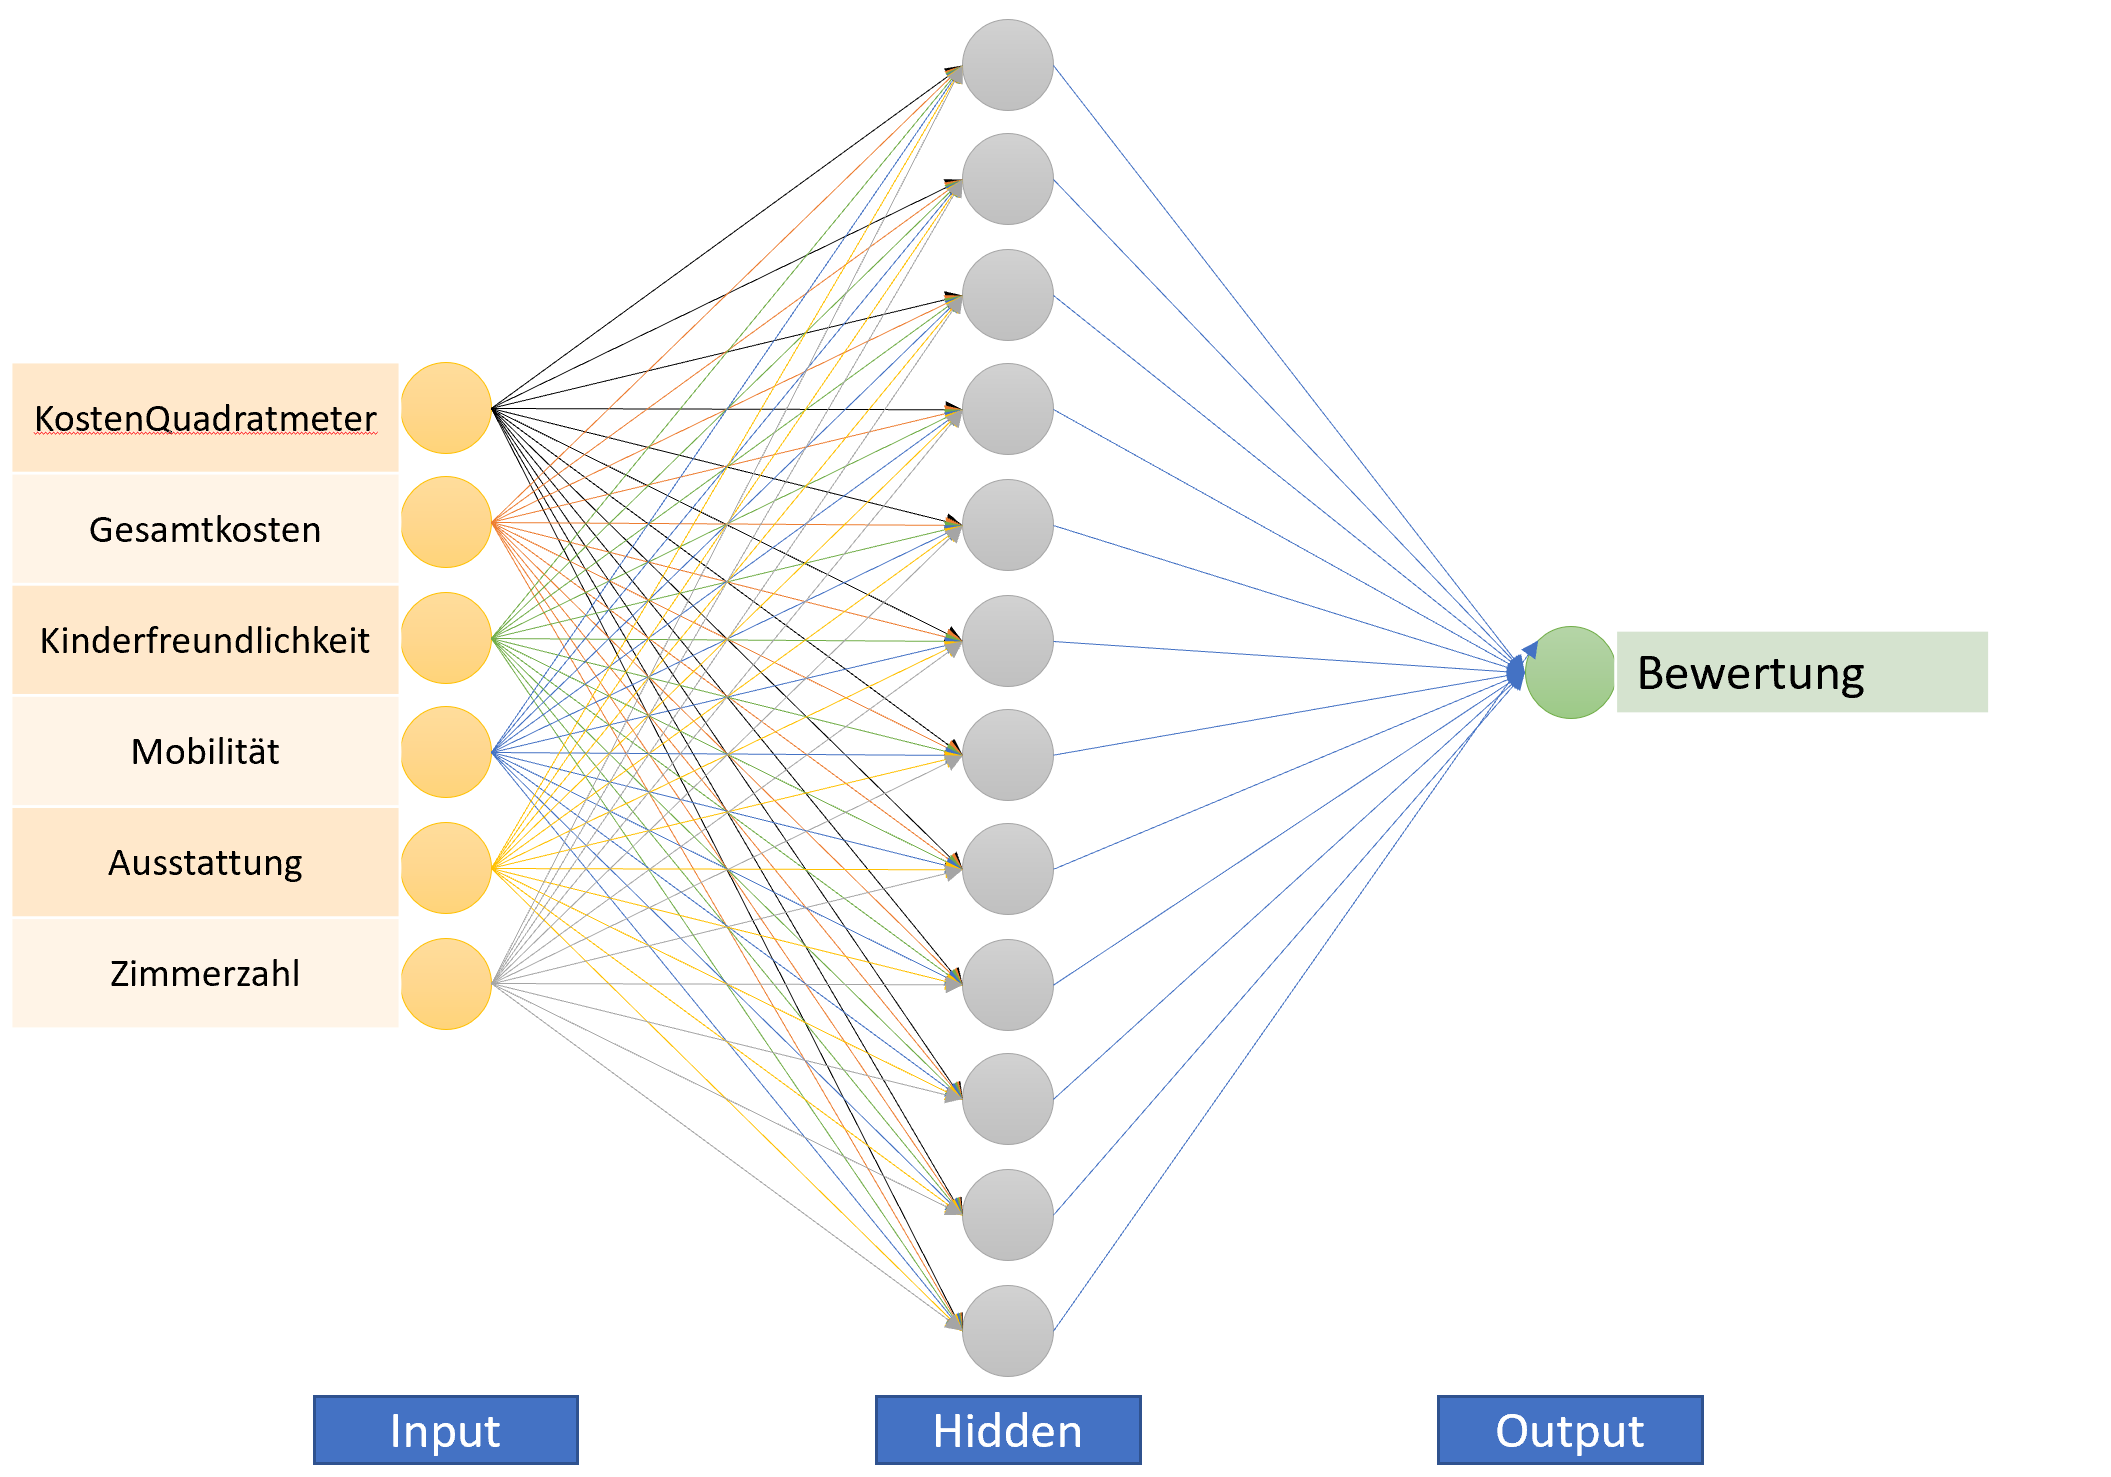
\includegraphics[width=15cm]{NNStruktur.PNG}
    \caption{Struktur des Neuronalen Netzes}
    \label{fig:nnStruktur}
\end{figure}

Die \textit{Input-Layer} besitzt $6$ Neuronen, dies entspricht der
Anzahl der Eigenschaften aus \autoref{lst:Eigenschaften}.
Die Anzahl der Neuronen in der \textit{Hidden-Layer} ergibt sich aus
$CountHidden = CountInput * 2$. Die \textit{Output-Layer} besitzt
lediglich ein Neuron, welches die Bewertung der Wohnung angibt.

\paragraph{Initiale Gewichtung der Neuronen}
Die initialen Gewichte für das Netz werden zufällig gesetzt. Diese werden in der Lernphase
mit Hilfe der Lernregel angepasst.

\paragraph{Aktivierungsfunktion und Schwellwert}
Die Aktivierungsfunktion eines Neurons gibt an, ab welchem Wert das Neuron das
einkommende Signal an die nächste Schicht weiterleitet.
Für diesen Anwendungsfall bietet sich eine Sigmoide-Funktion (\autoref{eqn:sigmoid}) an,
da diese die Eigenschaft besitzt ab dem Schwellwert allmählich
Signale weiterzuleiten.

Das bedeutet, ab einem Schwellwert von $0,5$, wird ein Signal weitergeleitet.
Allerdings erst bei einem Wert von $1$ ein maximales Signal.

\begin{equation}
    T_s(x) = \frac{1}{1+e^(\frac{x-S}{k})}
    \label{eqn:sigmoid}
\end{equation}

\paragraph{Lernregel}
Die Lernregel sorgt für die Anpassung der Gewichte. Das hier gewählte
Verfahren ist das \textit{Backpropagation-Verfahren}.
Es bietet sich an, da nach der Berechnung leicht der Netzfehler bestimmt werden kann.
Dieser Fehler wird anschließend zurück durch das Netz propagiert und die Gewichte
werden angepasst. Die Fehlerbestimmung erfolgt schichtweiße, beginnend mit der Output-Layer,
da hier der erwartete Wert zur Verfügung steht. Wurden die Fehler von jeder
Schicht bestimmt, werden die Gewichte angepasst.
Wie die Gewichte angepasst werden zeigt \autoref{eqn:gewichte}.
Hierbei wird das Gewicht des Neurons $j$ angepasst bei einer Eingabe,
von Neuron $i$. Der Fehler des aktuellen Neurons wird mit $\delta_j$ bezeichnet.
$x_i$ ist der Wert, welcher von $i$ an $j$ weitergegeben wird.
$\eta_i$ ist der Lernkoeffizient.
Dieser gibt an, wie stark die Gewichte angepasst werden und liegt zwischen 0 und 1.

\begin{equation}
    w_{ij}(t+1) = w_{ij}(t) + \eta * \delta_j*x_i
    \label{eqn:gewichte}
\end{equation}

Bei einfachen Problemen kann der Lernkoeffizent $=1$ sein.
Einerseits ist das hier beschriebene Problem nicht besonders einfach.
Andererseits sind nicht viele Schichten zur Lösung des Problems notwendig.
Daher bietet es sich an einen Lernkoeffizent von $0,7$ zu wählen.
Mit sinkendem Fehler kann dieser verringert werden,
um zu verhindern, dass die optimale Lösung \enquote{übersprungen} wird.

\subsection{Arbeitsweise/Ablauf}
Die folgende Auflistung zeigt, den Gesamtablauf des Netzes während eines
Lernschrittes.
\begin{enumerate}
    \item Initialisierung
    \item Berechnung der Aktivierung im \textit{Hidden-Layer}
    \item Berechnung Ausgabe der \textit{Hidden-Layer} mithilfe der Transferfunktion
    \item Berechnung Aktivierung im \textit{Output-Layer}
    \item Berechnung der Ausgabe durch die Transferfunktion.
    \item Berechnung des Fehlers der \textit{Output-Layer}
    \item Berechnung des Fehlers der \textit{Hidden-Layer}
    \item Berechnung des Fehlers der \textit{Input-Layer}
    \item Anpassung der Gewichte der \textit{Output-Layer}
    \item Anpassung der Gewichte der \textit{Hidden-Layer}
    \item Anpassung der Gewichte der \textit{Input-Layer}
\end{enumerate}
\section{Implementierung des Entscheidungsbaums}\label{sec:implementierung}
Das Programm implementiert den zuvor beschriebenen Algorithmus in der Programmiersprache Java.
Lediglich um Kommandozeilenparameter angenehmer einzupflegen wird eine Bibliothek verwendet.

\subsection{Ausführen des Programms}
\todoask[inline]{Anderer Dateiname?}
Im Anhang an diese Dokument befindet sich die Datei \enquote{tree.jar}.
Grundlegend kann das Programm, wie in \autoref{lst:jar-aufruf} gezeigt, aufgerufen werden.
Erforderlich ist hierfür zumindest Java in der Version 8.

\begin{lstlisting}[
    caption=Einfacher Aufruf des Programms,
    label=lst:jar-aufruf,
    language=bash
]
java -jar tree.jar
\end{lstlisting}

Durch verschiedene Parameter kann das Programm beeinflusst werden:
Die Parameter und ihre Standartwerte sind in folgdender Übersicht dargestellt.

\begin{description}
    \setlength\itemsep{-0.5em}
    \item[\texttt{-{}-teach, -t}]
        Datei, welche zum Trainieren genutzt wird\\
        Standard: \texttt{Wohnungskartei\_Muster\_Master\_5\_K\_teach.csv}
    \item[\texttt{-{}-check, -c}]
        Datei, welche mit dem Baum geprüft wird\\
        Standard: <leer>
    \item[\texttt{-{}-print, -p}]
        Wenn gesetzt, wird der Baum wie in \autoref{appendix:baum-training} dargestellt\\
        Standard: false
    \item[\texttt{-{}-default, -d}]
        Initiale Defaultwahrscheinlichkeit\\
        Standard: 0,5
    \item[\texttt{-{}-min-ratio, -r}]
        Mindestverhältnis zwischen Werten eines Attributs und Beispielmenge zur weiteren Unterteilung.\\
        Standard: 1
    \item[\texttt{-{}-use-saved-tree, -u}]
        Wenn gesetzt wird der Baum aus der angegebenen Datei geladen und nicht neu erzeugt.\\
        Standard: <leer>
    \item[\texttt{-{}-save-tree, -s}]
        Speichert den neu trainierten Baum in der angegebenen Datei.\\
        Standard: <leer>
    \item[\texttt{-{}-help}]
        Gibt die Hilfe in der Kommandozeile aus
\end{description}



\subsection{Besondere Aspekte}
\paragraph{Attribute}
Alle verfügbaren Attribute werden als \lstinline[language=Java]{enum} modelliert.
Jedes \lstinline[language=Java]{enum} gibt über die Funktion
\lstinline[language=Java]{getWerte()} die möglichen Ausprägungen als Liste von Zeichenketter zurück.

Auf diese Weise kann dass entsprechende Attribut as Parameter in Funktionsaufrufen übergeben werden und
innerhalb diese Funktion kann -- falls notwendig -- auf die möglichen Attributswerte zugegriffen werden.

\paragraph{Einlesen der Daten}
Weitestgehend werden die Daten direkt eingelesen und in ein \emph{Datensatz}-Objekt überführt.
Dieses Objekt enthält je ein Attribut für jedes der Merkmale und die Bewertung.
Für das Merkmal \enquote{Heizung} und für die Bewertung sind jedoch Schritte zur Vorverarbeitung notwendig:

Aus dem Zeichenketten \enquote{ja} und \enquote{nein} der Bewertung wird der entsprechende boolesche Wert ermittel.
In der Attributsausprägung \enquote{Lueftungsheizung} enthält der Datensatz anstatt des \textit{ue} ein undefiniertes Zeichen.
Dieses Problem wird dadurch gelöst, dass der Wert wie in \autoref{lst:heizung} angepasst wird.
Zwar wäre auch eine einmalige Änderung der entsprechende Werte in der Beispieldatei möglich,
die Programmzeile gestattet es aber auch, dass andere Dateien mit gleicher Formatierung bedenkenlos genutzt werden können.

\begin{lstlisting}[
    firstnumber=54,
    stepnumber=54,
    caption={Anpassen von \enquote{Heizung}},
    label=lst:heizung,
    language=Java
]
heizung = heizung.endsWith("ftungsheizung") ?
                    "Lueftungsheizung" :
                    heizung;
\end{lstlisting}

\paragraph{Datensatz}
Ein Datensatz-Objekt enthält für jeden relevanten Merkmalstyp eine Zeichenkette mit entsprechenden Namen.
Um dynamisch den Wert eines bestimmten Attributs zu erhalten kann dieses über die Funktion \lstinline[language=Java]{get()}
in \autoref{lst:datensatz-get} erfragt werden.

\lstinputlisting[
    caption={\texttt{get}-Funktion des Datensatzes (gekürzt)},
    label=lst:datensatz-get,
    language=Java
]{datensatz_get.java}

Für alle \enquote{normalen} Attribute wird der entsprechende Wert des Datensatzes zurückgegben.
Da die Bewertung ein boolescher Wert ist, die Funktion aber eine Zeichenkette zurückgeben muss,
wird dieser Wert entsprechend in eine Konstante umgewandelt.

\paragraph{Spezialisierung}
Das vorliegende Programm ist vor alle durch die Attribute und den Datensatz stark auf den gegebenen Anwendungsfall spezialisiert.
Theoretisch wäre es möglich ein Programm zu so konzipieren, dass es die Attribute und deren Wertemenge selbstständig aus den vorliegenden Daten extrahiert.
Dies würde jedoch die Komplexität und damit die Fehleranfälligkeit des Programms deutlich erhöhen.

\paragraph{Rekursionen}
Zum Erstellen des Baumes, aber auch zu Evaulation eines Datensatzes und zum Darstellen des Baumes wird Rekursion genutzt.
Beim Erstellen wird ein Attribut ausgewählt, und für jede Ausprägung ein Unterbaum nach gleiche Muster gebildet bis eine Enebedingung erreicht ist.
Details hierzu sind in \autoref{alg:baum-erzeugen} dargestellt.

Das \enquote{Ausdrucken} des Baums geschieht,
indem erst die Daten des aktuellen Knotens un
dann nach und nach die Daten der Unterbäume zu einer Zeichenkette hinzugefügt werden.

Um den Wert eines neuen Datensatzes zu ermitteln wird ausgehend von der Wurzel in jedem Knoten der zugehörige Attributswert aus dem Datensatz ausgelesen.
Dann wird die Bestimmungsfunktoin des zu diesem Wert zugehörige Unterbaums aufgerufen.
Dies geschieht rekursiv bis ein Blattknoten erreicht und damit der ermittelt ist.

\subsection{Test und Ergebnisbewertung}
Um den Algorithmus zu Testen und dessen Ergebnisse zu bewerten wird er in folgenden Konfigurationen ausgeführt:

\useunder{\uline}{\ul}{}
\begin{table}[h]
    \begin{center}
        \begin{tabular}{|l|l|l|l|}
        \hline
            {\ul \textbf{Nr.}} & {\ul \textbf{Trainingsdaten}} & {\ul \textbf{Testdaten}}      & {\ul \textbf{Verhältnis}} \\
            \hline
            1                  & \dots 5\_K\_teach.csv & \dots 4\_K.csv        & $0$ \\
            \hline
            2                  & \dots 5\_K\_teach.csv & \dots 4\_K.csv        & $1$ \\
            \hline
            3                  & \dots 5\_K\_teach.csv & \dots 4\_K.csv        & $2$ \\
            \hline
            \hline
            4                  & \dots 4\_K.csv        & \dots 5\_K\_teach.csv & $0$ \\
            \hline
            5                  & \dots 4\_K.csv        & \dots 5\_K\_teach.csv & $1$ \\
            \hline
            6                  & \dots 4\_K.csv        & \dots 5\_K\_teach.csv & $2$ \\
            \hline
        \end{tabular}
        \caption{Konfigurationen zur Ausführung}
        \label{tab:run-config}
    \end{center}
\end{table}

Die Genauigkeit der Klassifikation der jeweiligen Bäume wird bestimmt,
indem sowohl für die Trainings- als auch für die Testdaten eine Klassifikation ermittelt wird.
Die Ist-Klassifikation wird dann mit der Soll-Klassifikation verglichen.
Als Ergebnis wird der Anteil der korrekt Klassifizierten Datensätze herausgegeben.
Da das Ergebnis der Klassifikation eine Zahl zwischen $0$ und $1$ ist,
gilt jeder Wert $\geq 0.5$ als positive und jeder Wert $< 0.5$ als negative Klassifikation.
Es ergeben sich die in \autoref{tab:run-results} dargestellten Ergebnisse:

\todoask[inline]{
    Problem: Wenn Gültig $\geq 0.5$ ist, dann sind die Ergebnisse von 1 und 2 Gleich.\\
    Wenn Gültig nur $> 0.5$ ist, dann ist 1 mit 98,8\% schlechter (aber mann würde Werte mit 0.5 nie als "richtig" werten)\\
    Was ist besser?
}
\useunder{\uline}{\ul}{}
\begin{table}[h]
    \begin{center}
        \begin{tabular}{|l|l|l|l|}
        \hline
            {\ul \textbf{Nr.}} & {\ul \textbf{Ergebnis Trainingsdaten}} & {\ul \textbf{Ergebnis Testdaten}} \\
            \hline
            1                  & $100\%$                                & $\approx 98,901\%$                  \\
            \hline
            2                  & $99,75\%$                              & $\approx 98,901\%$                  \\
            \hline
            3                  & $99\%$                                 & $\approx 98,601\%$                  \\
            \hline
            \hline
            4                  & $100\%$                                & $98,5\%$                  \\
            \hline
            5                  & $100\%$                                & $98,5\%$                  \\
            \hline
            6                  & $\approx 99,4\%$                       & $97,5\%$                  \\
            \hline
        \end{tabular}
        \caption{Konfigurationen zur Ausführung}
        \label{tab:run-results}
    \end{center}
\end{table}


\todo[inline]{Beschreibung das Verhältnis 1 am besten ist }

Für Fall 2 ergibt sich der in \autoref{appendix:baum-training} dargestellte Baum.
Er zeigt folgende Eigenschaften der Trainingsdaten:
\begin{itemize}
    \item Für die Kunden ist es unumgänglich, dass die Wohnung in Schulnähe und nicht möbeliert ist.
    \item Es kommen nur Wohnungen zwischen 3-4 und 5 Zimmern in Frage.
    \item Bei 3-4 bis 4-5 Zimmern darf die Wohnung nicht zu weit von einem Kindergarten entfernt sein.
    \item Ist eine 4-5 Zimmerwohnung in erreichbarer Nähe eines Kindergartens, so sollte sie nicht nur ein Waschbecken enthalten.
    \item Bei 5 Zimmern darf die Wohnung zwischen nicht über 120 Quadratmeter groß sein.
\end{itemize}

Aus diesen Eigenschaften lässt sich Interpretieren,
dass der Kunde eine Familie mit Schul- und wahrscheinlich Kindergartenkind(ern) ist.
Hauptindizien hierfür sind, die Nähe zu Schule und Kingergarten, sowie die Zimmerzahl.


Betrachtet man den Baum von Fall 5 in \autoref{appendix:baum-test},
so finden sich diese Merkmale weitestgehen wieder.
Auch hier ist die Nähe zur Schule das wichtigste Merkmal.
Allerdings folgt dann die Zimmerzahl (wieder mit 3-4 bis 5 Zimmern).
Erst dann folgen - je nach Zimmerzahl in unterschiedlichen Reihenfolgen - die Kindergartennähe,
das Bad, und die Möbelierung.
Interesanterweiße kommen in zwei Fällen die Attribute Kaution beziehungweise die Art der Heizung hinzu.

\section{Fazit}\label{sec:fazit}
\subsection{Konzepte}
\paragraph{Neuronales Netz}
In diesem Programmentwurf wurde das Konzept für ein neuronales Netz vorgestellt, dass das Wohnungsbörsenproblem
löst. Bei einem Konzept für ein neuronales Netz ist die Vorverarbeitung ein sehr wichtiger und nicht zu vernachlässigender 
Schritt Der nächste Schritt ist es nun, dieses Konzept praktisch zu testen. Dies könnte beispielsweise mit der 
Python-Bibliothek \emph{Tensorflow} umgesetzt werden.
Tensorflow bietet verschiedene Methoden, mit deren Hilfe Deep Learning Systeme erstellt werden können.
Einige Parameter wie zum Beispiel die Lernrate können mithilfe der praktischen Umsetzung weiter optimiert werden. \\
Generell lässt sich feststellen, dass ein neuronales Netz die gegebene Problemstellung lösen kann. 

\subsection{Ergebnis und Implementierung}
\todo[inline]{Bin mir nicht sicher, ob die subsection-Einteilung so Sinn macht...}

Durch die Klassifikation eines Datensatzes werden Ergebnisse der Klassifikation untereinander vergleichbar.
So würde der Kunde (anhand der Trainingsdaten) eine  \emph{schulnahe, unmöbelierte, 4-5-Zimmer-Wohnung in erreichbarer Kindergartennähe mit Badewanne} wahrscheinlicher als positiv bewerten,
als eine \emph{schulnahe, unmöbelierte, 5-Zimmer-Wohung mit 71-80 Quadratmetern}.

Die \emph{Verhältnisoptimierung} wirkt einer Überanpassung des Baumes entgegen.
Zwar hat ein Mindestverhältnis von $1$ in den gegebenen Daten keinen Einfluss auf die Klassifikation der Testdaten und sogar einen negativen Einfluss auf die Trainingsdaten.
Allerdings zeigt sich beim direkten Verlgeich der Bäume,
dass durch das Verhältnis der Baum weniger tief und damit allgemeiner ist.

Allerdings kann diese Optimierung auch dazu führen,
dass alle Blattknoten eines Baumes das gleiche binäre Ergebnis liefern.
Ist lediglich eine binäre Klassifikation gewünscht,
so sollte der Baum nachträglich \enquote{gesäubert} werden,
um die spätere Klassifikation zu erleichtern.

Insgesamt zeigt die Implementierung und deren Ausführung mit den gegebenen Daten,
dass in allen Fällen - mit Ausnahme von C2 - die Testdaten mit über $98\%$ erfolgreich klassifiziert wurden.
Außerdem ist der \enquote{gedruckte} Baum für einen Menschen greifbar und einfach zu interpretieren.

%\printacronyms{}
\printbibliography{}


\newpage
\appendix
\section{Beispiel-Baum}
\lstinputlisting[
    caption=Beispiel-Baum,
    label=Python-Code
    language={}
]{beispielbaum.txt}
\end{document}
